\documentclass[12pt]{beamer}
\usepackage{../Estilos/BeamerMAF}
%Sección para el tema de beamer, con el theme, usercolortheme y sección de footers
\usetheme{CambridgeUS}
\usecolortheme{beaver}
%\useoutertheme{default}
\setbeamercovered{invisible}
% or whatever (possibly just delete it)
\setbeamertemplate{section in toc}[sections numbered]
\setbeamertemplate{subsection in toc}[subsections numbered]
\setbeamertemplate{subsection in toc}{\leavevmode\leftskip=3.2em\rlap{\hskip-2em\inserttocsectionnumber.\inserttocsubsectionnumber}\inserttocsubsection\par}
\setbeamercolor{section in toc}{fg=blue}
\setbeamercolor{subsection in toc}{fg=blue}
\setbeamercolor{frametitle}{fg=blue}
\setbeamertemplate{caption}[numbered]

\setbeamertemplate{footline}
\beamertemplatenavigationsymbolsempty
\setbeamertemplate{headline}{}


\makeatletter
\setbeamercolor{section in foot}{bg=gray!30, fg=black!90!orange}
\setbeamercolor{subsection in foot}{bg=blue!30!yellow, fg=red}
\setbeamercolor{date in foot}{bg=black, fg=white}
\setbeamertemplate{footline}
{
  \leavevmode%
  \hbox{%
  \begin{beamercolorbox}[wd=.333333\paperwidth,ht=2.25ex,dp=1ex,center]{section in foot}%
    \usebeamerfont{section in foot} \insertsection
  \end{beamercolorbox}%
  \begin{beamercolorbox}[wd=.333333\paperwidth,ht=2.25ex,dp=1ex,center]{subsection in foot}%
    \usebeamerfont{subsection in foot}  \insertsubsection
  \end{beamercolorbox}%
  \begin{beamercolorbox}[wd=.333333\paperwidth,ht=2.25ex,dp=1ex,right]{date in head/foot}%
    \usebeamerfont{date in head/foot} \insertshortdate{} \hspace*{2em}
    \insertframenumber{} / \inserttotalframenumber \hspace*{2ex} 
  \end{beamercolorbox}}%
  \vskip0pt%
}
\makeatother\newlength{\depthofsumsign}
\setlength{\depthofsumsign}{\depthof{$\sum$}}
\newcommand{\nsum}[1][1.4]{% only for \displaystyle
    \mathop{%
        \raisebox
            {-#1\depthofsumsign+1\depthofsumsign}
            {\scalebox
                {#1}
                {$\displaystyle\sum$}%
            }
    }
}
\def\scaleint#1{\vcenter{\hbox{\scaleto[3ex]{\displaystyle\int}{#1}}}}
\def\bs{\mkern-12mu}





\date{}
\title{Polinomios de Hermite - Ejercicio}
\author{M. en C. Gustavo Contreras Mayén}
\begin{document}
\maketitle
\fontsize{14}{14}\selectfont
\spanishdecimal{.}

\section*{Contenido}
\frame[allowframebreaks]{\tableofcontents[currentsection, hideallsubsections]}

%Referencia: Griffiths - Introduction to quantum mechanics. Cap. 2.3

\section{El oscilador armónico}
\frame{\tableofcontents[currentsection, hideothersubsections]}
\subsection{Caso clásico}

\begin{frame}
\frametitle{El oscilador clásico}
Sabemos que el oscilador armónico clásico consiste de una masa $m$ atada a un resorte con una constante $k$, el movimiento que describe la masa sigue la ley de Hooke:
\pause
\begin{align*}
    F = - k \, x = m \, \dv[2]{x}{t}
\end{align*}
\end{frame}
\begin{frame}
\frametitle{Solución al oscilador clásico}
Que tiene por solución (si omitimos la fricción)
\begin{align*}
    x(t) = A \, \sin (\omega \, t) + B \, \cos (\omega \, t)
\end{align*}
\pause
donde
\begin{align}
    \omega \equiv \sqrt{\dfrac{k}{m}}
    \label{eq:ecuacion_02_036}
\end{align}
es la frecuencia angular de oscilación.
\end{frame}
\begin{frame}
\frametitle{Energía en el oscilador}
La energía potencial correspondiente es
\begin{align}
    V(x) = \dfrac{1}{2} k \, x^{2}
    \label{eq:ecuacion_02_037}
\end{align}
cuyo trazo es el de una parábola.
\end{frame}
\begin{frame}
\frametitle{Consideraciones del oscilador}
De hecho, no existe como tal un oscilador armónico \emph{perfecto}: si estiramos demasiado el resorte, éste se romperá, por lo que la ley de Hooke ya no se cumple una vez que se alcanza este punto.
\end{frame}
\begin{frame}
\frametitle{Consideraciones del oscilador}
Podemos considerar que cualquier potencial es \textit{aproximadamente} parabólico en la vecindad de un mínimo local, como se puede ver en la figura (\ref{fig:figura_001}):
\end{frame}
\begin{frame}
\frametitle{Aproximación parabólica}
\begin{figure}[H]
    \centering
    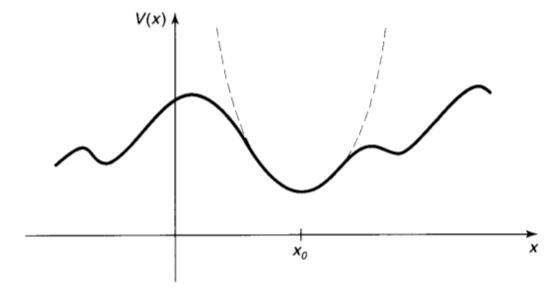
\includegraphics[scale=0.4]{Imagenes/Potencial_arbitrario.png}
    \caption{Aproximación parabólica (curva sesgada) en un potencial arbitrario, en la vecindad de un mínimo local.}
    \label{fig:figura_001}
\end{figure}
\end{frame}
\begin{frame}
\frametitle{Expandiendo la solución en una serie}
Es posible expandir el potencial $V(x)$ es una serie de Taylor alrededor del mínimo:
\begin{align*}
    V(x) = V(x_{0}) + \ptilde{V} (x_{0}) (x - x_{0}) + \dfrac{1}{2} \stilde{V} (x_{0}) (x - x_{0}) + \ldots
\end{align*}
\end{frame}
\begin{frame}
\frametitle{Resultado de la expansión en una serie}
Veamos que:
\setbeamercolor{item projected}{bg=blue!70!black,fg=yellow}
\setbeamertemplate{enumerate items}[circle]
\begin{enumerate}[<+->]
\item Es posible eliminar $V(x_{0})$, ya que podemos agregar una constante al potencial $V(x)$ y no modifica en nada a la fuerza.
\item Tenemos que $\ptilde{V}(x_{0}) = 0$, ya que $x_{0}$ es un mínimo local.
\item Podemos descartar los términos de orden superior, que se anulan mientras $(x - x_{0})$ se mantenga pequeño.
\end{enumerate}
\end{frame}
\begin{frame}
\frametitle{Sobre el potencial}
Por lo que el potencial se representa como
\begin{align*}
    V(x) \cong \dfrac{1}{2} \, \stilde{V} (x_{0}) (x - x_{0})^{2}
\end{align*}
que describe un oscilación armónica (alrededor de $x_{0}$), con una constante efectiva del resorte $k = \stilde{V} (x_{0}$).
\end{frame}
\begin{frame}
\frametitle{Sobre el potencial}
Considera que $\stilde{V}(x_{0})\geq 0$, tomando en cuenta de que $x_{0}$ es un mínimo local. En el extraño caso de que $\stilde{V} (x_{0})= 0$, la oscilación ya no se aproxima a la de un oscilador armónico.
\end{frame}
\begin{frame}
\frametitle{Relevancia del oscilador armónico}
Esta es la importancia del oscilador armónico: cualquier movimiento oscilatorio se puede aproximar a una oscilación armónica, mientras la amplitud sea pequeña.
\end{frame}

\section{El oscilador cuántico}
\frame{\tableofcontents[currentsection, hideothersubsections]}
\subsection{Planteamiento}

\begin{frame}
\frametitle{El oscilador cuántico}
El problema cuántico es resolver la ecuación de Schrödinger para el potencial
\begin{align}
    V(x) = \dfrac{1}{2} m \, \omega^{2} \, x^{2}
    \label{eq:ecuacion_02_038}
\end{align}
\end{frame}
\begin{frame}
\frametitle{El oscilador cuántico}
Por lo que la ecuación de Schrödinger independiente del tiempo es
\begin{align}
    - \dfrac{\hbar}{2 m} \dv[2]{\psi}{x} + \dfrac{1}{2} m \, \omega \, x^{2} \, \psi = E \, \psi
    \label{eq:ecuacion_02_039}
\end{align}
\end{frame}
\begin{frame}
\frametitle{Enfoques para resolver el problema}
En la literatura se encontrarán dos enfoques completamente diferentes para resolver este problema.
\setbeamercolor{item projected}{bg=blue!70!black,fg=yellow}
\setbeamertemplate{enumerate items}[circle]
\begin{enumerate}[<+->]
\item El primero es una solución de \enquote{fuerza bruta} directa a la ecuación diferencial, que utiliza el método de expansión en una serie de potencias; tiene la virtud de que la misma estrategia se puede aplicar a muchos otros potenciales.
\item El segundo es una técnica algebraica \emph{ingeniosa}, que utiliza los llamados \textbf{operadores de escalera}.
\end{enumerate}
\end{frame}

\subsection{Método analítico.}

\begin{frame}
\frametitle{La ecuación de Schrödinger}
Regresamos nuevamente a la ecuación de Schrödinger para el oscilador armónico (ec. \ref{eq:ecuacion_02_039})
\begin{align*}
- \dfrac{\hbar}{2 m} \dv[2]{\psi}{x} + \dfrac{1}{2} m \, \omega \, x^{2} \, \psi = E \, \psi  
\end{align*}
\end{frame}
\begin{frame}
\frametitle{Haciendo un cambio de variable}
Para un desarrollo más claro, hacemos el siguiente cambio de variable adimensional
\begin{align}
\xi \equiv \sqrt{ \dfrac{m \omega}{\hbar}} \, x
    \label{eq:ecuacion_02_055}
\end{align}
\end{frame}
\begin{frame}
\frametitle{La ecuación con el cambio de variable}
Por lo que en términos de $\xi$, la ecuación de Schrödinger toma la forma:
\begin{align}
\dv[2]{\psi}{\xi} = (\xi^{2} - K) \, \psi
    \label{eq:ecuacion_02_056}
\end{align}
donde $K$ es la energía, \pause en unidades de $(1/2) \hbar \omega$:
\begin{align}
K \equiv \dfrac{2 \, E}{\hbar \, \omega}
    \label{eq:ecuacion_02_057}
\end{align}
\end{frame}
\begin{frame}
\frametitle{Problema a resolver}
Nuestro problema es resolver la ec. (\ref{eq:ecuacion_02_056}):
\begin{align*}
\dv[2]{\psi}{\xi} = (\xi^{2} - K) \, \psi
\end{align*}
\pause
y durante el proceso obtener los valores \enquote{permitidos} de $K$ (y por tanto de $E$).
\end{frame}
\begin{frame}
\frametitle{Analizando los valores}
Para iniciar, veamos que para valores muy grandes de $\xi$ (que a la vez, es decir que tendríamos valores muy grandes de $x$), el término $\xi^{2}$ domina sobre la constante $K$, por lo que tendríamos:
\pause
\begin{align}
\dv[2]{\psi}{\xi} \approx \xi^{2} \, \psi
    \label{eq:ecuacion_02_058}
\end{align}
\end{frame}
\begin{frame}
\frametitle{Solución al caso}
Que tiene por solución
\begin{align}
\psi (\xi) \approx A \, \exp \left( - \dfrac{\xi^{2}}{2} \right) + B \, \exp \left( + \dfrac{\xi^{2}}{2} \right)
    \label{eq:ecuacion_02_059}
\end{align}
\end{frame}
\begin{frame}
\frametitle{Normalización de términos}
En donde encontramos que el término $B$ no se puede normalizar (no funciona cuando $\abs{x} \to \infty$), por lo que las soluciones aceptables con sentido físico, tienen las forma asintótica:
\pause
\begin{align}
\psi (\xi) = ( \quad ) \exp \left( - \dfrac{\xi^{2}}{2} \right) \hspace{1cm} \text{con valores grandes de } \xi
    \label{eq:ecuacion_02_060}
\end{align}
\end{frame}
\begin{frame}
\frametitle{Aprovechando términos}
Esto sugiere que \enquote{aprovechamos} la parte exponencial:
\pause
\begin{align}
    \psi (\xi) = h (\xi) \, \exp \left( - \dfrac{\xi^{2}}{2} \right)
    \label{eq:ecuacion_02_061}
\end{align}
Esperando que lo que queda de $[h (\xi)]$ tenga una forma funcional más simple que $\psi (\xi)$ mismo.
\end{frame}
\begin{frame}
\frametitle{Removiendo comportamientos asintóticos}
Toma en cuenta que aunque invocamos algunas aproximaciones para motivar la ec. (\ref{eq:ecuacion_02_061}), lo que sigue es exacto.
\\
\bigskip
\pause
La técnica para eliminar el comportamiento asintótico es el primer paso estándar en el método de la serie de potencias para resolver ecuaciones diferenciales.
\end{frame}
\begin{frame}
\frametitle{Construyendo la expresión}
Diferenciando la ec. (\ref{eq:ecuacion_02_061}), se tiene que:
\pause
\begin{align*}
    \dv{\psi}{\xi} = \left( \dv{h}{\xi} - \xi \, h \right) \, \exp \left( - \dfrac{\xi^{2}}{2} \right)
\end{align*}
\end{frame}
\begin{frame}
\frametitle{Construyendo la expresión}
Por lo que la ec. de Schrödinger (ec. \ref{eq:ecuacion_02_056}) es:
\pause
\begin{align}
    \dv[2]{h}{\xi} - 2 \, \xi \, \dv{h}{\xi} +  (K - 1) \, h = 0
    \label{eq:ecuacion_02_062}
\end{align}
\end{frame}
\begin{frame}
\frametitle{Propuesta de solución}
Proponemos una solución a la ED (\ref{eq:ecuacion_02_062}) en la forma de una serie de potencias en $\xi$:
\begin{align}
    h (\xi) = a_{0} + a_{1} \, \xi + a_{2} \, \xi^{2} + \ldots = \sum_{j=0}^{\infty} a_{j} \, \xi^{j}
    \label{eq:ecuacion_02_063}
\end{align}
\end{frame}
\begin{frame}
\frametitle{Resolviendo por series}
Diferenciamos en dos ocasiones la solución para obtener
\begin{align*}
\dv{h}{\xi} &= \sum_{j=0}^{\infty} j \, a_{j} \, \xi^{j-1} \\[0.5em]
\dv[2]{h}{\xi} &= \sum_{j=0}^{\infty} (j + 1)(j + 2) \, a_{j+2} \, \xi^{j}
\end{align*}
\end{frame}
\begin{frame}
\frametitle{Resolviendo por series}
Que al sustituir en la ec. (\ref{eq:ecuacion_02_062}), tenemos que:
\pause
\begin{align}
\sum_{j=0}^{\infty} \bigg[ (j + 1)(j + 2) \, a_{j+2} - 2 \, j \, a_{j} +  (K - 1) \, a_{j} \bigg] \, \xi^{j} = 0
\label{eq:ecuacion_02_64}
\end{align}
\end{frame}
\begin{frame}
\frametitle{Anulando coeficientes}
Sabemos que los coeficientes para cada potencia de $\xi$ deben de anularse, por tanto:
\pause
\begin{align*}
(j + 1)(j + 2) \, a_{j+2} - 2 \, j \, a_{j} +  (K - 1) \, a_{j} = 0
\end{align*}
\pause
de donde se obtiene que
\begin{align}
a_{j+2} = \dfrac{(2 \, j + 1 - K)}{(j + 1)(j + 2)} \, a_{j}
\label{eq:ecuacion_02_065}
\end{align}
\end{frame}
\begin{frame}
\frametitle{Regla de recurrencia}
Esta es la \textbf{regla de recurrencia}:
\begin{align*}
a_{j+2} = \dfrac{(2 \, j + 1 - K)}{(j + 1)(j + 2)} \, a_{j}
\end{align*}
\pause
que es en sí misma, equivalente a la ecuación de Schrödinger.
\end{frame}
\begin{frame}
\frametitle{Obteniendo los coeficientes}
Dado $a_{0}$, podemos obtener $a_{2}, a_{4}, a_{6}, \ldots$, también para un $a_{1}$ dado, podemos obtener los $a_{3}, a_{5}, a_{7}, \ldots$
\end{frame}
\begin{frame}
\frametitle{Obteniendo los coeficientes}
Podemos escribir entonces:
\begin{align}
h (\xi) = h_{\text{par}} (\xi) + h_{\text{impar}} (\xi)
\label{eq:ecuacion_02_066}
\end{align}
\end{frame}
\begin{frame}
\frametitle{Obteniendo los coeficientes}
Donde:
\begin{align*}
h_{\text{par}} (\xi) = a_{0} + a_{2} \, \xi^{2} + a_{4} \, \xi^{4} + \ldots
\end{align*}
si es una función par de $\xi$ (ya que involucra sólo potencias pares) a partir de $a_{0}$, \pause y como
\begin{align*}
h_{\text{impar}} (\xi) = a_{1} \, \xi + a_{3} \, \xi^{3} + a_{5} \, \xi^{5} + \ldots
\end{align*}
si es función impar, a partir de $a_{1}$.
\end{frame}
\begin{frame}
\frametitle{Constantes necesarias}
Entonces tenemos que la ec. (\ref{eq:ecuacion_02_065}) determina a $h(\xi)$ en términos de dos constantes arbitrarias ($a_{0}$ y $a_{1}$), que es lo que se esperaba.
\end{frame}
\begin{frame}
\frametitle{Solución aproximada}
Dado que tenemos una ED2:
\pause
\begin{align*}
a_{j+2} \approx \dfrac{2}{j} \, a_{j}
\end{align*}
\pause
con una solución (aproximada)
\begin{align*}
a_{j} \approx \dfrac{C}{(j/2)!}
\end{align*}
para alguna constante $C$.
\end{frame}
\begin{frame}
\frametitle{Solución aproximada}
Esto nos lleva a (para valores grandes de $\xi$, donde las potencias elevadas dominan)
\pause
\begin{align*}
h (\xi) \approx C \sum \dfrac{1}{(j/2)!} \, \xi^{j} \approx C \sum \dfrac{1}{k!} \xi^{2 k} \approx C \, \exp \left( \xi^{2} \right)
\end{align*}
\end{frame}
\begin{frame}
\frametitle{Comportamiento no deseado}
Veamos ahora lo siguiente: si $h \to \exp \left( \xi^{2} \right)$, entonces ¿$\psi \to \exp \left( \xi^{2}/2 \right)$?, por que presenta un comportamiento asintótico que no se desea!
\\
\bigskip
\pause
Solo hay una forma de salir de esto: para soluciones normalizables, \textit{la serie de potencias debe terminar}.
\end{frame}
\begin{frame}
\frametitle{Cota mayor de términos}
Debe de presentarse un valor \enquote{mayor} de $j$ (llámalo $n$) de manera que la fórmula de recursión devuelva un $a_{n+2} = 0$ (esto truncará cada una de las series par o impar; la otra debe ser cero desde el principio). 
\end{frame}
\begin{frame}
\frametitle{Soluciones consistentes ocn la física}
Para soluciones físicamente aceptables, entonces, debemos tener que
\begin{align*}
    K = 2 \, n + 1
\end{align*}
para un entero positivo $n$.
\end{frame}
\begin{frame}
\frametitle{La energía en el oscilador}
Es decir (refiriéndose a la ecuación (\ref{eq:ecuacion_02_057})) que la energía debe ser de la forma:
\pause
\begin{align}
E_{n} = \left( n + \dfrac{1}{2} \right) \, \hbar \, \omega , \hspace{1.5cm} n = 0, 1, 2, \ldots
\label{eq:ecuacion_02_067}
\end{align}
\pause
Así recuperamos, mediante un método completamente diferente, la condición fundamental de cuantificación que con el método algebraico.
\end{frame}
\begin{frame}
\frametitle{Resultado consistente}
Para los valores permitidos de $K$, la fórmula de recurrencia es:
\begin{align}
a_{j+2} = - \dfrac{2 (n - j)}{(j + 1)(j + 2)} \, a_{j}
\label{eq:ecuacion_02_068}
\end{align}
\end{frame}
\begin{frame}
\frametitle{Elección de los primeros coeficientes}
Si $n = 0$, hay sólo un término en la serie (debemos de escoger $a_{1} = 0$ para cancelar $h_{\text{impar}}$ y $j=0$ en la ec. (\ref{eq:ecuacion_02_068}), nos lleva a $a_{2}=0$):
\pause
\begin{align*}
h_{0} (\xi) = a_{0}
\end{align*}
\end{frame}
\begin{frame}
\frametitle{Con $n=0$ y $n=1$}
Por lo tanto:
\pause
\begin{align*}
\psi_{0} (\xi) = a_{0} \, \exp \left( - \dfrac{\xi^{2}}{2} \right)
\end{align*}
\\
\bigskip
\pause
Para $n=1$, escogemos $a_{0} = 0$ y la ec. (\ref{eq:ecuacion_02_068}) con $j = 1$, nos devuelve $a_{3} = 0$, así:
\pause
\begin{align*}
h_{1} (\xi) = a_{1} \, \xi
\end{align*}
\end{frame}
\begin{frame}
\frametitle{Con $n=1$ y $n=2$}
Por lo que:
\pause
\begin{align*}
\psi_{1} (\xi) = a_{1} \, \xi \, \exp \left( - \dfrac{\xi^{2}}{2} \right)
\end{align*}
\\
\bigskip
\pause
Para $n = 2$, $j = 0$, tenemos que $a_{2} = - 2 \, a_{0}$ y $j = 2$ nos da que $a_{4} = 0$ por lo tanto:
\pause
\begin{align*}
h_{2} (\xi) = a_{0} (1 - 2 \, \xi^{2})
\end{align*}
\end{frame}
\begin{frame}
\frametitle{Resultado con $n=2$}
Entonces:
\pause
\begin{align*}
\psi_{2} (\xi) = a_{0} (1 - 2 \, \xi^{2}) \, \exp \left( - \dfrac{\xi^{2}}{2} \right)
\end{align*}

y así sucesivamente.
\end{frame}
\begin{frame}
\frametitle{Resultado general}
En general, $h_{n} (\xi)$ será un polinomio de grado $n$ en $\xi$, que involucra sólo las potencias pares, si $n$ es un entero par, y las potencias impares solamente, si $n$ es un entero impar.
\\
\bigskip
\pause
Aparte del factor global $(a_{0}$ o $a_{1})$, se tienen los llamados \textbf{polinomios de Hermite}, $H_{n} (\xi)$.
\end{frame}
\begin{frame}
\frametitle{Polinomios de Hermite}
Los primeros polinomios de Hermite se muestran en la siguiente tabla: %(\ref{tabla_001}).
%\begin{center}
\begin{table}[H]
\centering
\begin{tabular}{l l}
$H_{0} =$ & $1$ \\
$H_{1} =$ & $2 \, x$ \\
$H_{2} =$ & $4 \, x^{2} - 2 $ \\
$H_{3} =$ & $8 \, x^{3} - 12 \, x$ \\
$H_{4} =$ & $16 \, x^{4} - 48 \, x^{2} + 12 $ %\\
%$H_{5} =$ & $32 \, x^{5} - 160 \, x^{3} + 120 \, x $
\end{tabular}
%\caption{Primeros polinomios de Hermite $H_{n}(x)$.}
\label{tabla_001}
\end{table}
\end{frame}
\begin{frame}
\frametitle{Gráfica de los polinomios de Hermite}
\begin{figure}[H]
    \centering
    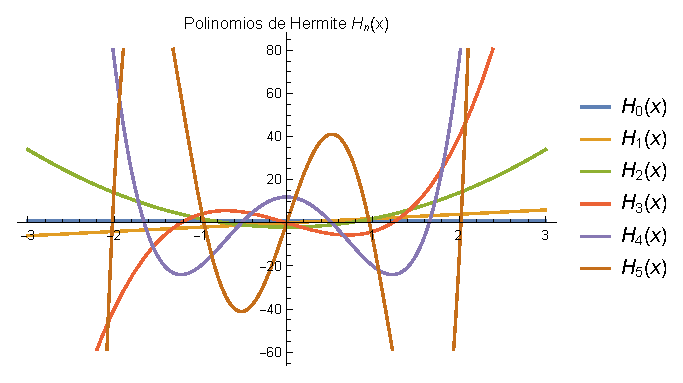
\includegraphics[scale=1]{Imagenes/Plot_Hermite.eps}
    \caption{Gráfica de los primeros polinomios de Hermite.}
    \label{figura_003}
\end{figure}
\end{frame}
\begin{frame}
\frametitle{Factor multiplicativo}
Por tradición, el factor multiplicativo arbitrario se elige de modo que el coeficiente de la potencia más alta de $\xi$ es $2^{n}$.
\end{frame}
\begin{frame}
\frametitle{Estador normalizados}
Con esta convención, los estados estacionarios normalizados para el oscilador armónico son
\begin{align}
\psi_{n} (x) = \left( \dfrac{m \, \omega}{\pi \, \hbar} \right)^{1/4} \, \dfrac{1}{\sqrt{2^{n} \, n!}} \, H_{n} (\xi) \, \exp \left( - \dfrac{\xi^{2}}{2} \right)
\label{eq:ecuacion_02_069}
\end{align}
\end{frame}

\section{Propiedades de los Polinomios de Hermite}
\frame{\tableofcontents[currentsection, hideothersubsections]}
\subsection{Algunas propiedades}

\begin{frame}
\frametitle{Revisión breve}
Las propiedades de los polinomios de Hermite se obtienen a partir de la definición y como en algunas otras funciones especiales, a partir de la función generatriz.
\\
\bigskip
\pause
Mencionaremos algunas propiedades para resolver un ejercicio.
\end{frame}
\begin{frame}
\frametitle{Normalización de los polinomios de Hermite}
La normalización de los polinomios ha sido elegida de modo tal que 
\begin{align*}
H_{0}(x) = 1
\end{align*}
\end{frame}
\begin{frame}
\frametitle{Relaciones de recurrencia}
Algunas relaciones de recurrencia para los polinomios de Hermite son:
\begin{align*}
H_{n+1} (x) &= 2 \, x \, H_{n} (x) - 2 \, n \, H_{n-1} (x) \\
\dot{H}_{n} (x) &= 2 \, n \, H_{n-1} \\
H_{n} (x) &= (-)^{n} \, H_{n} (-x) \\
H_{2n} (0) &= (-)^{n} \, \dfrac{(2 \, n)!}{n!} \\
H_{2n+1} (0) &= 0
\end{align*}
\end{frame}
\begin{frame}
\frametitle{Ortogonalidad}
La condición de ortogonalidad es:
\begin{align*}
\int_{-\infty}^{\infty} e^{-x^{2}} \, H_{n} (x) \, H_{m} (x) \dd{x} = 2^{n} \, \sqrt{\pi} \, n! \, \delta_{m n}
\end{align*}
Con $n = 0, 1, 2, \ldots$
\end{frame}

\section{Ejercicio con los \texorpdfstring{$H_{n}(x)$}{Hn(x)}}
\frame{\tableofcontents[currentsection, hideothersubsections]}
\subsection{Transición de probabilidad entre dos estados}

\begin{frame}
\frametitle{Ejercicio}
La transición de probabilidad entre dos estados $\psi_{m}$ y $\psi_{n}$ del oscilador armónico cuántico depende de que el valor de la siguiente integral sea:
\begin{align*}
\int_{-\infty}^{\infty} x \, e^{-x^{2}} \, H_{n}(x) \, &H_{m}(x) \dd{x} = \sqrt{\pi} \, 2^{n-1} \, n! \, \delta_{m,n-1} \\[1em]
&+ \sqrt{\pi} \, 2^{n} \, (n+1)! \, \delta_{m,n+1}
\end{align*}
\pause
\textbf{Obtén explícitamente este valor.}
\end{frame}

\subsection{Solución}

\begin{frame}
\frametitle{Resolviendo el ejercicio}
La solución de este ejercicio se basa en ocupar algunas de las propiedades de los polinomios de Hermite:
\pause
\setbeamercolor{item projected}{bg=blue!70!black,fg=yellow}
\setbeamertemplate{enumerate items}[circle]
\begin{enumerate}[<+->]
\item Relaciones de recurrencia.
\item Condición de ortogonalidad.
\end{enumerate}
\end{frame}
\begin{frame}
\frametitle{Usando una relación de recurrencia}
De la relación de recurrencia:
\pause
\begin{align*}
H_{n+1} (x) &= 2 \, x \, H_{n} (x) - 2 \, n \, H_{n-1} (x)
\end{align*}
\pause
tenemos que:
\begin{align*}
x \, H_{n} (x) = n \, H_{n-1} (x) + \dfrac{1}{2} H_{n+1} (x)
\end{align*}
\end{frame}
\begin{frame}
\frametitle{Reexpresando la integral}
Ocupando el resultado anterior, reescribimos la integral:
\pause
\begin{align*}
&\scaleint{5ex}_{\bs -\infty}^{\infty} x \, e^{-x^{2}} \, H_{n}(x) \, H_{m}(x) \dd{x} = \\[0.5em]
&= \scaleint{5ex}_{\bs -\infty}^{\infty} e^{-x^{2}} H_{m}(x) \bigg[ n \, H_{n-1} (x) + \dfrac{1}{2} H_{n+1} (x) \bigg] \dd{x}
\end{align*}
\pause
que separamos en dos integrales.
\end{frame}
\begin{frame}
\frametitle{Resolviendo dos integrales}
\begin{eqnarray*}
&= \scaleint{5ex}_{\bs -\infty}^{\infty} e^{-x^{2}} H_{m}(x) \bigg[ n \, H_{n-1} (x) + \dfrac{1}{2} H_{n+1} (x) \bigg] \dd{x} = \\[0.5em] \pause
&= n \, \scaleint{5ex}_{\bs -\infty}^{\infty} e^{-x^{2}} \, H_{n-1} (x) \, H_{m}(x) \dd{x} + \\[0.5em]
&+ 2^{-1} \, \scaleint{5ex}_{\bs -\infty}^{\infty} e^{-x^{2}} \, H_{n+1} (x) \, H_{m}(x) \dd{x}
\end{eqnarray*}
\end{frame}
\begin{frame}
\frametitle{Usando la ortogonalidad de la base}
Como la base $\left\{ H_{n}(x) \right\}$ es ortogonal, tal que la condición es:
\begin{align*}
\scaleint{5ex}_{\bs -\infty}^{\infty} e^{-x^{2}} \, H_{n} (x) \, H_{m} (x) \dd{x} = 2^{n} \, \sqrt{\pi} \, n! \, \delta_{m n}
\end{align*}
\pause
tendremos que las integrales son:
\end{frame}
\begin{frame}
\frametitle{Resultado de las integrales}
La primera integral es:
\pause
\begin{align*}
n \scaleint{5ex}_{\bs -\infty}^{\infty} e^{x^{2}} H_{n-1} (x) H_{m}(x) \dd{x} &= n \, 2^{n-1} \, \sqrt{\pi} \, (n {-} 1)! \, \delta_{m, n-1} \\[0.5em]
&= \sqrt{\pi} \, 2^{n-1} \, n! \, \delta_{m, n-1}
\end{align*}
\end{frame}
\begin{frame}
\frametitle{Resultado de las integrales}
La segunda integral es:
\pause
\begin{align*}
2^{-1} \scaleint{5ex}_{\bs -\infty}^{\infty} e^{x^{2}} H_{n+1} (x) &H_{m}(x) \dd{x} = \\[0.5em]
&= 2^{-1} \cdot 2^{n+1} \sqrt{\pi} (n {+} 1)! \delta_{m,n+1} = \\[0.5em]
&= \sqrt{\pi} \, 2^{n} \, (n {+} 1)! \, \delta_{m,n+1}
\end{align*}
\end{frame}
\begin{frame}
\frametitle{Resultado completo}
Se demuestra entonces que:
\begin{align*}
&\scaleint{5ex}_{\bs -\infty}^{\infty} x e^{-x^{2}} H_{n}(x) H_{m}(x) \dd{x} = \sqrt{\pi} \, 2^{n-1} \, n! \, \delta_{m,n-1} + \\[1em]
&+ \sqrt{\pi} \, 2^{n} \, (n+1)! \, \delta_{m,n+1} \qed
\end{align*}
\end{frame}
\end{document}